\documentclass[a4paper]{article}
\usepackage{graphicx}

\begin{document}

	\title{\Huge{Software Requirement Specification}}
	\author{Group 8}
	\maketitle

	\section{Introduction}

		The purpose of this document is to present a detailed description for the mark record and tracking solution. It will explain the purpose and features of the system, what the system will do, as well as the constraints under which it must operate. This document is intended as an official contract between the stakeholders and developers of the system.

	\section{Vision}

		The software solution will be aimed at providing a means for markers in a practical session to record student marks from a mobile device. The purpose is to allow for more efficient marking process, from initial recording of marks to the feedback of results for both lecturer and student. The system should manage recorded marks while ensuring proper authorization to any access of the data it contains. There would be three different user responsibilities, namely: lecturer, marker, and student.
		
		\subsection{Lecturer}
			\begin{itemize}
				\item	Full access to create, read, update and delete data within the lecturer's subject(s).
				\item	Ability to define practical sessions and associate mark allocations to these sessions.
				\item	Ability to open and close the mark inputs for practical sessions.
				\item	Ability to assign markers to practical sessions to enable access to data entry according to a time slot.
				\item	All activity on the system is logged for accountability during auditing.
				\item	Compiling of reports from practical marks.
			\end{itemize}

		\subsection{Marker}
			\begin{itemize}
				\item	Greater efficiency at locating the appropriate student for marking through search functionality.
				\item	Recording marks according to mark sheet set up by lecturer.
				\item	Having a centralized marking environment from which all responsibilities as a marker are accessible.
			\end{itemize}

		\subsection{Student}
			\begin{itemize}
				\item	Faster access to marks progress.
				\item	Ability to view track record and performance.
				\item	Provides accountability of markers involved during mark queries.
			\end{itemize}

	\section{Background}

		Currently the marking process is performed using physical documents. It is required of the marker to obtain a mark sheet from the lecturer, on which the student identification is paired with the results from the practical session. The data is then captured by a third party. This system lacks in accountability and efficiency which can be solved through a software solution and eliminating the need of a third party. The likelihood of marks being lost would also decrease as the data transfer process is diminished from a three step process (marker $\rightarrow$ entry $\rightarrow$ lecturer) to a direct process (marker $\rightarrow$ lecturer). As a result, students would also be able to receive quicker feedback on their work.

	\section{Architectural Requirements}

		\subsection{Access Channel Requiremnets}

			\begin{itemize}

				\item{An Item}

				\item{Another Item}

			\end{itemize}

		\subsection{Quality Requirements}

			\begin{enumerate}

				\item{An Item}

				\item{Another Item}

			\end{enumerate}

		\subsection{Integration Requirements}

			\begin{description}

				\item[first]{An Item}

				\item[second]{Another Item}

			\end{description}

		\subsection{Architecture Constraints}
		
			\subsubsection{Technologies}
		
				\begin{itemize}

					\item{Client interface must run on an Android device}

					\item{Client interface must be accessible through a web browser}
					
					\item{MySQL database must be used to store application data}
					
					\item{Python must be used in order to accommodate existing systems}

				\end{itemize}
				
			\subsubsection{Frameworks}
			
				\begin{itemize}

					\item{The application must be able to interface with the Django framework}

				\end{itemize}

	\section{Functional Requirements}

		\subsection{Introduction}

			This section introduces the functional requirements of the system, as seen by the different stakeholders:

			\subsubsection{Student}
				\begin{flushleft}
				A person who participates in examinable activities, for whom marks are recorded in the system. \linebreak 
				
				Students can:
				\end{flushleft}
				\begin{itemize}

					\item{View Marks}

				\end{itemize}

			\subsubsection{Marker}
				\begin{flushleft}
				A person who is responsible for grading a student, and who has to record marks for all students who he/she has graded. \linebreak 
				
				Markers can:
				\end{flushleft}
				\begin{itemize}

					\item{Input student marks}
					
					\item{View session marks}
					
					\item{Search for student}

				\end{itemize}
				
			\subsubsection{Lecturer}
				\begin{flushleft}
				A person who is responsible for setting examinable activities, as well as the logistics and administration of a particular course. \linebreak 
				
				Lecturers can:
				\end{flushleft}
				\begin{itemize}

					\item{Edit student marks}
					
					\item{View all marks}
					
					\item{Search for student}
					
					\item{Generate reports}
					
					\item{Assign system functions to Markers}
					
					\item{Create and edit marksheets}

				\end{itemize}
			
			\subsection{Scope and Limitations/Exclusions}
			\begin{figure}[h]
				\caption{High Level Use Case Diagram}
				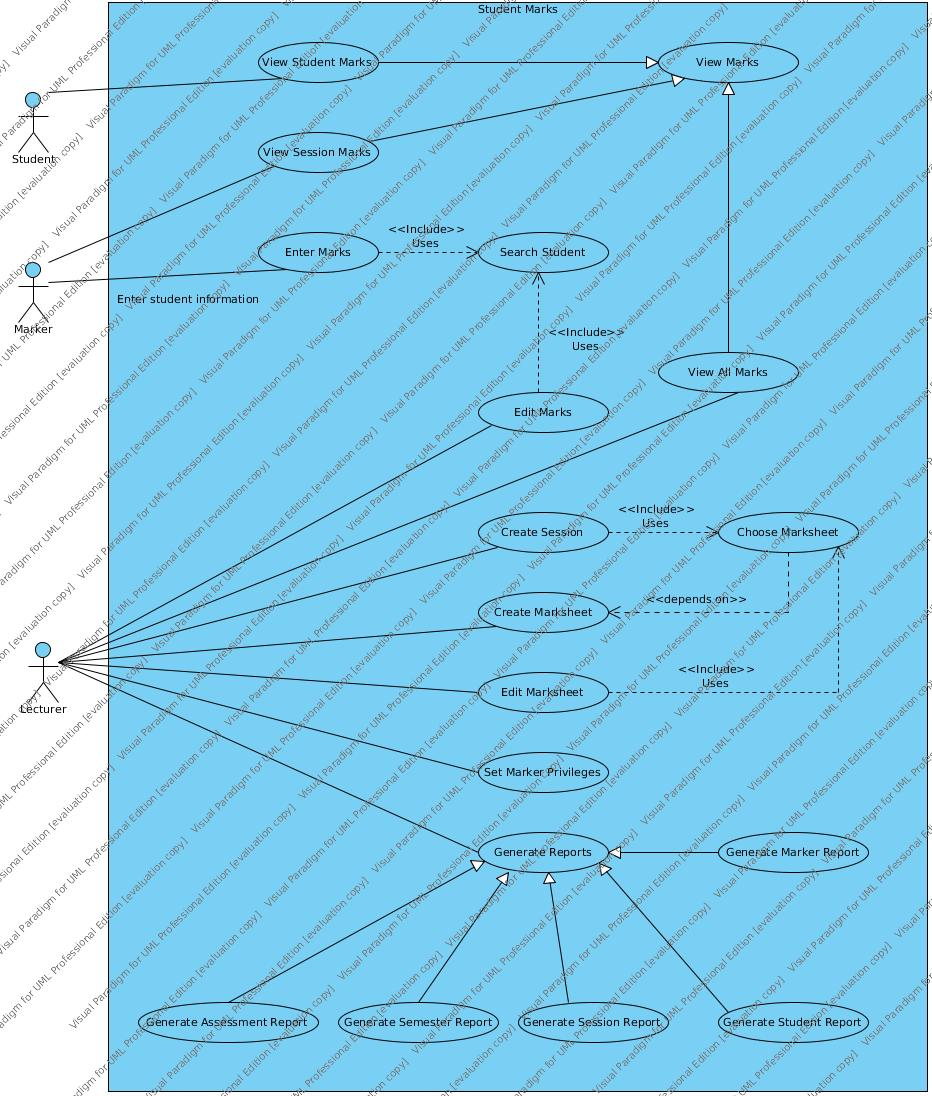
\includegraphics[height=10cm]{StudentMarks}
			\end{figure}

		\subsection{Required Functionality}
		\begin{enumerate}
		\item The system will have a Web and Android application.
		\item The system will have a search panel in which a user types in a student's details (student number/ name/ surname) with auto-complete functionality and displays that will show all possible results of the search.
		\item The system will retrieve the relevant information of a student depending on the access rights said user is granted.
		\item The system shall allow the recording and editing of marks by lecturers and markers.
		\item The system will have a history trail of all edits made to existing marks in the database.
		\item The system aims to provide real-time updates of marks to the database and if this is not possible due to unforseen circumstances, the system will have the option to update information on a smartphone's local storage first.
		\item The system will provide the following security features:
		\begin{itemize}
			\item{Check validity of user attempting to edit before granting access to edit marks.}
			\item{Automatic log off of a user if the system is not in use for more than 15 minutes.}
			\item{Automatic lock after a practical session.}
			\item{Log-in interface to restrict access to the students enrolled, markers and lecturers involved.}
			\item{User authentication checks}
			\item{Students will only be able to view their own marks and no other students' marks when logged in.}
			\item{Markers will only be able to view students in their session}
			\item{Only lecturers and markers will be granted access to enter marks into the database.}
			\item{Only lecturers will obtain a list of all the marks.}
		
		\end{itemize}
		
		\item The system will sanitize the input entered, i.e it will display an error message if the input is invalid.
		\item When entering marks the system will validate if the student is booked for the session.
		\item The system will allow only a lecturer to create a session, assign markers to groups of students and set marker priveleges.
		\item The system will have a reporting functionality that will provide the lecturer with statistics and visual reports such as graphs (distribution, bar), pie charts, average marks, median, mode and standard deviation. 
		\item The system will provide documents in .csv format as exports of marks to lecturers.
		
		\end{enumerate}
			\begin{figure}[h]
				\caption{Low Level Use Case Diagrams- Log In}
			%	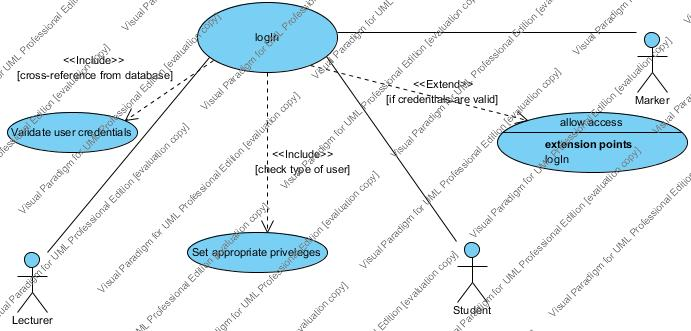
\includegraphics[height=7cm]{logIn}
			\end{figure}
			\begin{figure}[h]
				\caption{Create Session}
			%	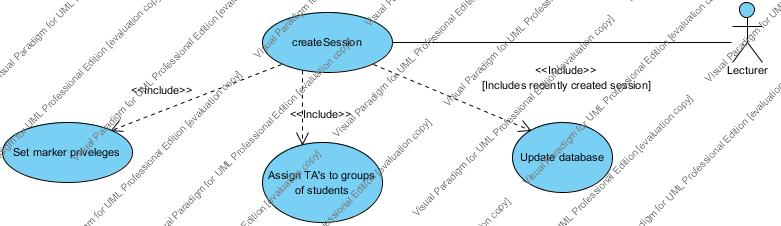
\includegraphics[height=7cm]{createSession}
			\end{figure}
			\begin{figure}[h]
				\caption{View Marks}
			%	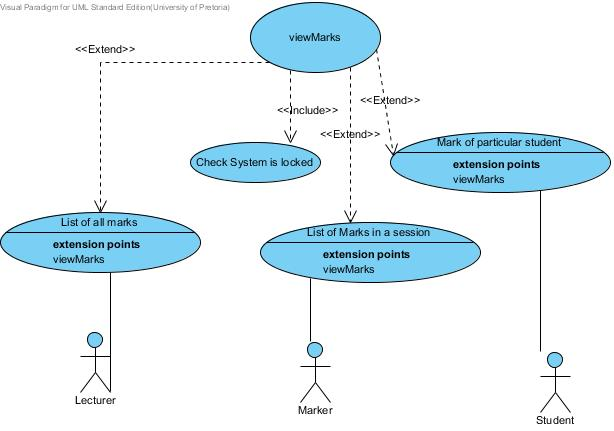
\includegraphics[height=7cm]{viewMarks}
			\end{figure}
			\begin{figure}[h]
				\caption{Generate Report}
			%	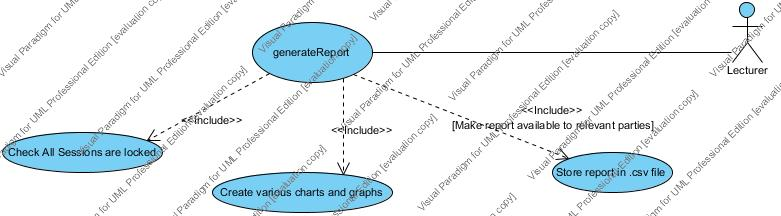
\includegraphics[height=7cm]{generateReport}
			\end{figure}
			\begin{figure}[h]
				\caption{Enter Marks}
			%	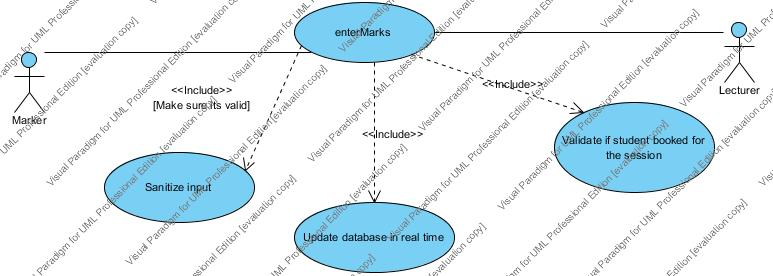
\includegraphics[height=7cm]{enterMarks}
			\end{figure}
			\begin{figure}[h]
				\caption{Edit Marks}
			%	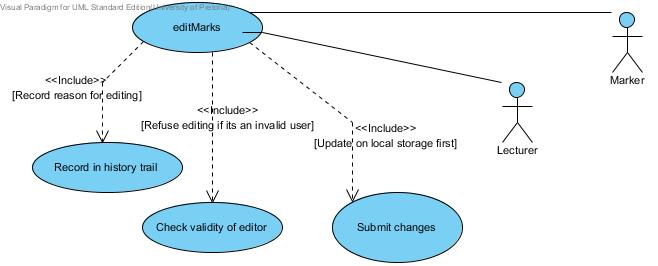
\includegraphics[height=7cm]{editMarks}
			\end{figure}
			\begin{figure}[h]
				\caption{Search Student}
			%	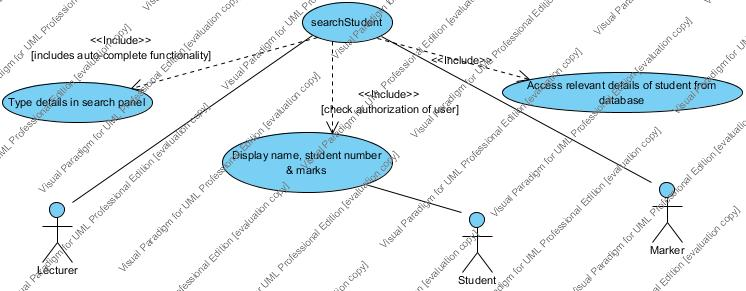
\includegraphics[height=7cm]{searchStudent}
			\end{figure}

		\subsection{Use Case Prioritisation}

		\subsection{Use Case/Service Contracts}

		\subsection{Process Specification}

		\subsection{Domain Objects}

	\section{Open Issues}

	\section{Glossary}

\end{document}
